\documentclass[11pt,letterpaper]{article}
\usepackage[utf8]{inputenc}
\usepackage{amsmath}
\usepackage{amsfonts}
\usepackage{amssymb}
\usepackage{makeidx}
\usepackage{graphicx}
\usepackage{lmodern}
\usepackage[left=2cm,right=2cm,top=2cm,bottom=2cm]{geometry}
\author{Argha Mondal}
\title{Vectorial Superposition}
\begin{document}

\maketitle
Starting with the vector potential:
\begin{equation}
\vec{A} = \frac{1}{\sqrt{2}}\left[ A_{n,\nu} J_{n}(j_{n,\nu}\frac{r}{R}) 
e^{in\phi} e^{i(kz\cos \alpha _{n} - \omega t)} + A_{n\prime,\nu \prime} 
J_{n\prime}(j_{n\prime,\nu \prime}\frac{r}{R}) e^{in\phi} 
e^{i(kz\cos \alpha _{n\prime} - \omega t)} \right] \hat{z}
\end{equation}
We use the following equation to calculate the electric field:
\begin{equation}
\vec{E} = ik\left[\vec{A} + \frac{1}{k^2}\bigtriangledown (\bigtriangledown \cdot \vec{A})\right]
\end{equation}
In cylindrical coordinate:
\begin{equation}
\vec{E_r} = \frac{i}{\sqrt{2}k}\left[ C_{n,\nu}(J_{n-1}(\varrho) 
- J_{n+1}(\varrho)) e^{in\phi}e^{i(kz\cos \alpha _n - \omega t)} +
C_{n\prime,\nu \prime}(J_{n\prime-1}(\varrho) - J_{n\prime+1}(\varrho))
e^{in\prime\phi}e^{i(kz\cos \alpha _{n\prime} - \omega t)}\right] \hat{r}
\end{equation}
,where $C_{n,\nu} = A_{n,\nu}ik\cos \alpha _{n}\frac{j_{n,\nu}}{2R}$, 
$\varrho = j_{n,\nu}\frac{r}{R}$, and $\alpha _{n} = \arccos \left( 
\sqrt{1-\frac{j_{n,\nu}^2}{k^2 R^2}}\right)$
\begin{equation}
\vec{E_{\phi}} = -\frac{i}{\sqrt{2}r}\left[ A_{n,\nu}n\cos \alpha _{n} 
J_{n}(\varrho)e^{in\phi}e^{i(kz\cos \alpha _{n} - \omega t)} + 
A_{n\prime,\nu \prime}n\prime \cos \alpha _{n\prime} J_{n\prime}(\varrho)
e^{in\prime \phi}e^{i(kz\cos \alpha _{n\prime} - \omega t)}\right] \hat{\phi}
\end{equation}
\begin{equation}
\vec{E_{z}} = \frac{ik}{\sqrt{2}}\left[ A_{n,\nu}\sin ^{2}\alpha _{n} 
J_{n}(\varrho)e^{in\phi}e^{i(kz\cos \alpha _{n} - \omega t)} + 
A_{n\prime,\nu \prime}\sin ^{2}\alpha _{n \prime} J_{n \prime}(\varrho)
e^{in\prime \phi}e^{i(kz\cos \alpha _{n\prime} - \omega t)} \right] \hat{z}
\end{equation}
Say $\Delta n = |n - n\prime|$. If $\Delta n = 1$ and $n = 10$ we have the following dynamics of $\rho(\vec{r},t) = |E_r(\vec{r})|^2$,

\begin{figure}
\centering
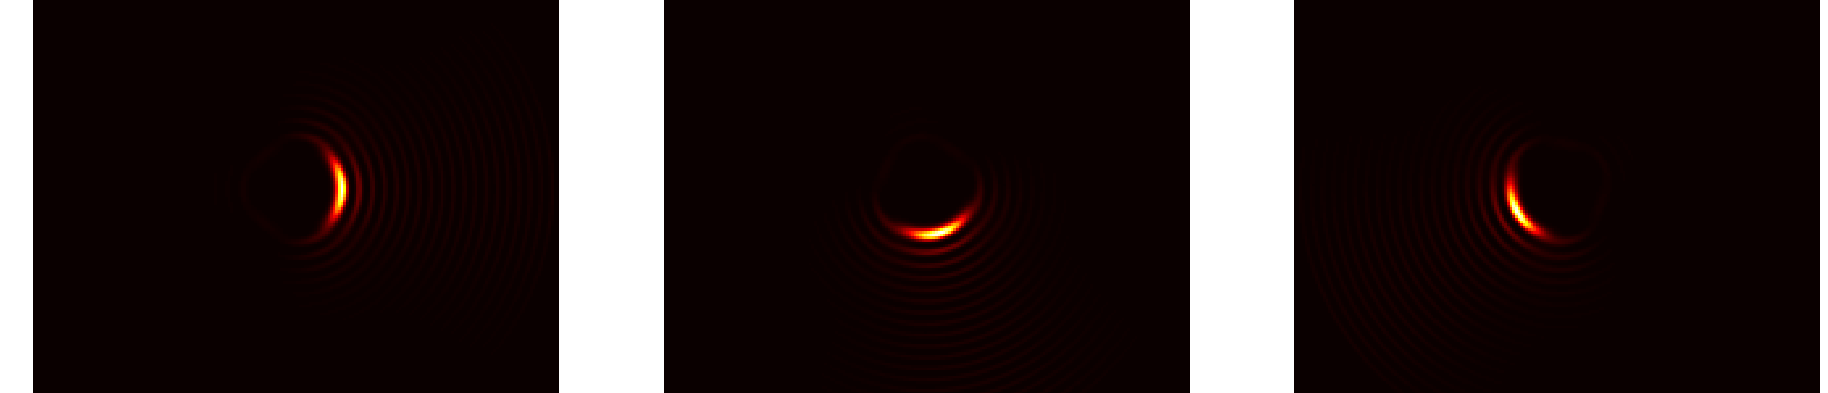
\includegraphics[scale=0.25]{pic2.png}
\caption{If $\Delta n = 1$ and $n = 10$ we have the dynamics as shown above.}
\end{figure}
\end{document}